%% fig_moduli.tex   (generated by make_diagrams.py; do not edit by hand)
%% The Weil family inside the moduli of principally polarised abelian 2n-folds: n^2 against n(2n+1), for n up to six.
\documentclass[tikz,border=8pt]{standalone}
\usepackage{amsmath,amssymb}
\usetikzlibrary{arrows.meta,calc}
%% palette.tex -- shared colour definitions for the figures
\definecolor{PInk}{RGB}{26,32,44}
\definecolor{PBlue}{RGB}{37,82,139}
\definecolor{PTeal}{RGB}{23,127,125}
\definecolor{POchre}{RGB}{193,138,44}
\definecolor{PClay}{RGB}{178,74,58}
\definecolor{PSlate}{RGB}{108,122,137}
\definecolor{PViolet}{RGB}{110,86,150}
\definecolor{WBlue}{RGB}{223,234,246}
\definecolor{WTeal}{RGB}{220,238,236}
\definecolor{WOchre}{RGB}{250,240,218}
\definecolor{WClay}{RGB}{247,229,224}
\definecolor{WSlate}{RGB}{238,241,244}
\definecolor{PMag}{RGB}{158,58,110}
\definecolor{PGrass}{RGB}{62,124,66}
\definecolor{PAmber}{RGB}{214,112,38}
\definecolor{PIndigo}{RGB}{58,64,140}
\definecolor{PRule}{RGB}{176,186,197}

%% shared macros so the standalone figures match the paper
\providecommand{\QQ}{\mathbb{Q}}
\providecommand{\ZZ}{\mathbb{Z}}
\providecommand{\RR}{\mathbb{R}}
\providecommand{\CC}{\mathbb{C}}
\providecommand{\PP}{\mathbb{P}}
\providecommand{\Kx}{K^{\times}}
\providecommand{\HW}{W}
\providecommand{\Nm}{\mathrm{N}}
\providecommand{\Hdg}{\mathrm{Hdg}}
\providecommand{\NS}{\mathrm{NS}}
\providecommand{\cA}{\mathcal{A}}
\providecommand{\cD}{\mathcal{D}}
\providecommand{\cF}{\mathcal{F}}
\providecommand{\cP}{\mathcal{P}}
\providecommand{\cO}{\mathcal{O}}
\providecommand{\cQ}{\mathcal{Q}}
\providecommand{\bbar}[1]{\overline{#1}}
\providecommand{\ch}{\operatorname{ch}}
\providecommand{\End}{\mathrm{End}}
\providecommand{\Ext}{\operatorname{Ext}}
\providecommand{\Supp}{\operatorname{Supp}}

\begin{document}
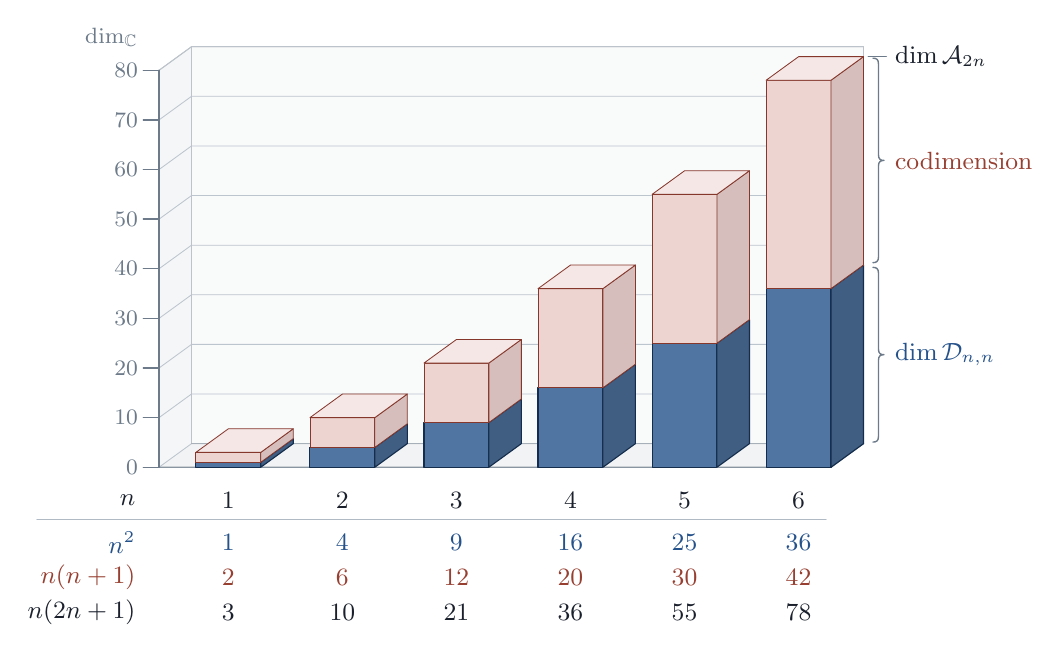
\begin{tikzpicture}[x=1cm,y=1cm,line join=round,line cap=round,
  font=\small,text=PInk]
  \path[fill=PSlate!9] (0.0000,0.0000) -- (8.5342,0.0000) -- (8.9473,0.3001) -- (0.4131,0.3001) -- cycle;
  \path[fill=PSlate!4] (0.4131,0.3001) -- (8.9473,0.3001) -- (8.9473,5.3411) -- (0.4131,5.3411) -- cycle;
  \path[fill=PSlate!7] (0.0000,0.0000) -- (0.4131,0.3001) -- (0.4131,5.3411) -- (0.0000,5.0410) -- cycle;
  \draw[PRule!85,line width=0.3pt] (0.0000,0.0000) -- (0.4131,0.3001) -- (8.9473,0.3001);
  \draw[PRule!85,line width=0.3pt] (0.0000,0.6301) -- (0.4131,0.9303) -- (8.9473,0.9303);
  \draw[PRule!85,line width=0.3pt] (0.0000,1.2602) -- (0.4131,1.5604) -- (8.9473,1.5604);
  \draw[PRule!85,line width=0.3pt] (0.0000,1.8904) -- (0.4131,2.1905) -- (8.9473,2.1905);
  \draw[PRule!85,line width=0.3pt] (0.0000,2.5205) -- (0.4131,2.8206) -- (8.9473,2.8206);
  \draw[PRule!85,line width=0.3pt] (0.0000,3.1506) -- (0.4131,3.4508) -- (8.9473,3.4508);
  \draw[PRule!85,line width=0.3pt] (0.0000,3.7807) -- (0.4131,4.0809) -- (8.9473,4.0809);
  \draw[PRule!85,line width=0.3pt] (0.0000,4.4109) -- (0.4131,4.7110) -- (8.9473,4.7110);
  \draw[PRule!85,line width=0.3pt] (0.0000,5.0410) -- (0.4131,5.3411) -- (8.9473,5.3411);
  \draw[PSlate!45,line width=0.35pt] (0.0000,5.0410) -- (0.4131,5.3411) -- (8.9473,5.3411) -- (8.9473,0.3001);
  \draw[PSlate!45,line width=0.35pt] (0.4131,0.3001) -- (0.4131,5.3411);
  \draw[PSlate!60,line width=0.4pt] (0.4131,0.3001) -- (8.9473,0.3001);
  \draw[PSlate!80,line width=0.45pt] (0.0000,0.0000) -- (8.5342,0.0000) -- (8.9473,0.3001);
  \draw[PSlate,line width=0.5pt] (0.0000,0.0000) -- (0.0000,5.0410);
  \draw[PSlate,line width=0.5pt] (0.0000,0.0000) -- (-0.1988,0.0000);
  \draw[PSlate,line width=0.5pt] (0.0000,0.6301) -- (-0.1988,0.6301);
  \draw[PSlate,line width=0.5pt] (0.0000,1.2602) -- (-0.1988,1.2602);
  \draw[PSlate,line width=0.5pt] (0.0000,1.8904) -- (-0.1988,1.8904);
  \draw[PSlate,line width=0.5pt] (0.0000,2.5205) -- (-0.1988,2.5205);
  \draw[PSlate,line width=0.5pt] (0.0000,3.1506) -- (-0.1988,3.1506);
  \draw[PSlate,line width=0.5pt] (0.0000,3.7807) -- (-0.1988,3.7807);
  \draw[PSlate,line width=0.5pt] (0.0000,4.4109) -- (-0.1988,4.4109);
  \draw[PSlate,line width=0.5pt] (0.0000,5.0410) -- (-0.1988,5.0410);
  \path[fill=PBlue!80,draw=PBlue!55!black,line width=0.4pt] (0.4686,0.0000) -- (1.2922,0.0000) -- (1.2922,0.0630) -- (0.4686,0.0630) -- cycle;
  \path[fill=PBlue!80!white!80!black,draw=PBlue!55!black,line width=0.4pt] (1.2922,0.0000) -- (1.7053,0.3001) -- (1.7053,0.3632) -- (1.2922,0.0630) -- cycle;
  \path[fill=PClay!24,draw=PClay!75!black,line width=0.3pt] (0.4686,0.0630) -- (1.2922,0.0630) -- (1.2922,0.1890) -- (0.4686,0.1890) -- cycle;
  \path[fill=PClay!24!white!90!black,draw=PClay!75!black,line width=0.3pt] (1.2922,0.0630) -- (1.7053,0.3632) -- (1.7053,0.4892) -- (1.2922,0.1890) -- cycle;
  \path[fill=PClay!13,draw=PClay!75!black,line width=0.3pt] (0.4686,0.1890) -- (1.2922,0.1890) -- (1.7053,0.4892) -- (0.8817,0.4892) -- cycle;
  \path[fill=PBlue!80,draw=PBlue!55!black,line width=0.4pt] (1.9170,0.0000) -- (2.7406,0.0000) -- (2.7406,0.2520) -- (1.9170,0.2520) -- cycle;
  \path[fill=PBlue!80!white!80!black,draw=PBlue!55!black,line width=0.4pt] (2.7406,0.0000) -- (3.1537,0.3001) -- (3.1537,0.5522) -- (2.7406,0.2520) -- cycle;
  \path[fill=PClay!24,draw=PClay!75!black,line width=0.3pt] (1.9170,0.2520) -- (2.7406,0.2520) -- (2.7406,0.6301) -- (1.9170,0.6301) -- cycle;
  \path[fill=PClay!24!white!90!black,draw=PClay!75!black,line width=0.3pt] (2.7406,0.2520) -- (3.1537,0.5522) -- (3.1537,0.9303) -- (2.7406,0.6301) -- cycle;
  \path[fill=PClay!13,draw=PClay!75!black,line width=0.3pt] (1.9170,0.6301) -- (2.7406,0.6301) -- (3.1537,0.9303) -- (2.3301,0.9303) -- cycle;
  \path[fill=PBlue!80,draw=PBlue!55!black,line width=0.4pt] (3.3654,0.0000) -- (4.1890,0.0000) -- (4.1890,0.5671) -- (3.3654,0.5671) -- cycle;
  \path[fill=PBlue!80!white!80!black,draw=PBlue!55!black,line width=0.4pt] (4.1890,0.0000) -- (4.6021,0.3001) -- (4.6021,0.8673) -- (4.1890,0.5671) -- cycle;
  \path[fill=PClay!24,draw=PClay!75!black,line width=0.3pt] (3.3654,0.5671) -- (4.1890,0.5671) -- (4.1890,1.3233) -- (3.3654,1.3233) -- cycle;
  \path[fill=PClay!24!white!90!black,draw=PClay!75!black,line width=0.3pt] (4.1890,0.5671) -- (4.6021,0.8673) -- (4.6021,1.6234) -- (4.1890,1.3233) -- cycle;
  \path[fill=PClay!13,draw=PClay!75!black,line width=0.3pt] (3.3654,1.3233) -- (4.1890,1.3233) -- (4.6021,1.6234) -- (3.7785,1.6234) -- cycle;
  \path[fill=PBlue!80,draw=PBlue!55!black,line width=0.4pt] (4.8138,0.0000) -- (5.6374,0.0000) -- (5.6374,1.0082) -- (4.8138,1.0082) -- cycle;
  \path[fill=PBlue!80!white!80!black,draw=PBlue!55!black,line width=0.4pt] (5.6374,0.0000) -- (6.0505,0.3001) -- (6.0505,1.3083) -- (5.6374,1.0082) -- cycle;
  \path[fill=PClay!24,draw=PClay!75!black,line width=0.3pt] (4.8138,1.0082) -- (5.6374,1.0082) -- (5.6374,2.2684) -- (4.8138,2.2684) -- cycle;
  \path[fill=PClay!24!white!90!black,draw=PClay!75!black,line width=0.3pt] (5.6374,1.0082) -- (6.0505,1.3083) -- (6.0505,2.5686) -- (5.6374,2.2684) -- cycle;
  \path[fill=PClay!13,draw=PClay!75!black,line width=0.3pt] (4.8138,2.2684) -- (5.6374,2.2684) -- (6.0505,2.5686) -- (5.2269,2.5686) -- cycle;
  \path[fill=PBlue!80,draw=PBlue!55!black,line width=0.4pt] (6.2622,0.0000) -- (7.0858,0.0000) -- (7.0858,1.5753) -- (6.2622,1.5753) -- cycle;
  \path[fill=PBlue!80!white!80!black,draw=PBlue!55!black,line width=0.4pt] (7.0858,0.0000) -- (7.4989,0.3001) -- (7.4989,1.8755) -- (7.0858,1.5753) -- cycle;
  \path[fill=PClay!24,draw=PClay!75!black,line width=0.3pt] (6.2622,1.5753) -- (7.0858,1.5753) -- (7.0858,3.4657) -- (6.2622,3.4657) -- cycle;
  \path[fill=PClay!24!white!90!black,draw=PClay!75!black,line width=0.3pt] (7.0858,1.5753) -- (7.4989,1.8755) -- (7.4989,3.7658) -- (7.0858,3.4657) -- cycle;
  \path[fill=PClay!13,draw=PClay!75!black,line width=0.3pt] (6.2622,3.4657) -- (7.0858,3.4657) -- (7.4989,3.7658) -- (6.6753,3.7658) -- cycle;
  \path[fill=PBlue!80,draw=PBlue!55!black,line width=0.4pt] (7.7106,0.0000) -- (8.5342,0.0000) -- (8.5342,2.2684) -- (7.7106,2.2684) -- cycle;
  \path[fill=PBlue!80!white!80!black,draw=PBlue!55!black,line width=0.4pt] (8.5342,0.0000) -- (8.9473,0.3001) -- (8.9473,2.5686) -- (8.5342,2.2684) -- cycle;
  \path[fill=PClay!24,draw=PClay!75!black,line width=0.3pt] (7.7106,2.2684) -- (8.5342,2.2684) -- (8.5342,4.9150) -- (7.7106,4.9150) -- cycle;
  \path[fill=PClay!24!white!90!black,draw=PClay!75!black,line width=0.3pt] (8.5342,2.2684) -- (8.9473,2.5686) -- (8.9473,5.2151) -- (8.5342,4.9150) -- cycle;
  \path[fill=PClay!13,draw=PClay!75!black,line width=0.3pt] (7.7106,4.9150) -- (8.5342,4.9150) -- (8.9473,5.2151) -- (8.1237,5.2151) -- cycle;
  \draw[PSlate,line width=0.5pt] (9.0673,0.3201) .. controls (9.1093,0.3201) and (9.1373,0.3341) .. (9.1373,0.3901) -- (9.1373,1.3594) .. controls (9.1373,1.4154) and (9.1653,1.4294) .. (9.2073,1.4294) .. controls (9.1653,1.4294) and (9.1373,1.4434) .. (9.1373,1.4994) -- (9.1373,2.4686) .. controls (9.1373,2.5246) and (9.1093,2.5386) .. (9.0673,2.5386);
  \draw[PSlate,line width=0.5pt] (9.0673,2.5986) .. controls (9.1093,2.5986) and (9.1373,2.6126) .. (9.1373,2.6686) -- (9.1373,3.8269) .. controls (9.1373,3.8829) and (9.1653,3.8969) .. (9.2073,3.8969) .. controls (9.1653,3.8969) and (9.1373,3.9109) .. (9.1373,3.9669) -- (9.1373,5.1251) .. controls (9.1373,5.1811) and (9.1093,5.1951) .. (9.0673,5.1951);
  \draw[PSlate,line width=0.5pt] (9.0073,5.2151) -- (9.2373,5.2151);
  \draw[PRule,line width=0.4pt] (-1.5500,-0.6600) -- (8.4724,-0.6600);
  \node[text=PSlate,font=\footnotesize,inner sep=0pt] at (-0.343,0.000) {$0$};
  \node[text=PSlate,font=\footnotesize,inner sep=0pt] at (-0.418,0.630) {$10$};
  \node[text=PSlate,font=\footnotesize,inner sep=0pt] at (-0.418,1.260) {$20$};
  \node[text=PSlate,font=\footnotesize,inner sep=0pt] at (-0.418,1.890) {$30$};
  \node[text=PSlate,font=\footnotesize,inner sep=0pt] at (-0.418,2.520) {$40$};
  \node[text=PSlate,font=\footnotesize,inner sep=0pt] at (-0.418,3.151) {$50$};
  \node[text=PSlate,font=\footnotesize,inner sep=0pt] at (-0.418,3.781) {$60$};
  \node[text=PSlate,font=\footnotesize,inner sep=0pt] at (-0.418,4.411) {$70$};
  \node[text=PSlate,font=\footnotesize,inner sep=0pt] at (-0.418,5.041) {$80$};
  \node[text=PSlate,font=\footnotesize,inner sep=0pt] at (-0.603,5.461) {$\dim_{\CC}$};
  \node[text=PBlue,font=\small,inner sep=0pt] at (9.982,1.434) {$\dim\cD_{n,n}$};
  \node[text=PClay!85!black,font=\small,inner sep=0pt] at (10.220,3.892) {codimension};
  \node[text=PInk,font=\small,inner sep=0pt] at (9.930,5.215) {$\dim\cA_{2n}$};
  \node[text=PInk,font=\small,inner sep=0pt] at (-0.398,-0.420) {$n$};
  \node[text=PInk,font=\small,inner sep=0pt] at (0.880,-0.420) {$1$};
  \node[text=PInk,font=\small,inner sep=0pt] at (2.329,-0.420) {$2$};
  \node[text=PInk,font=\small,inner sep=0pt] at (3.777,-0.420) {$3$};
  \node[text=PInk,font=\small,inner sep=0pt] at (5.226,-0.420) {$4$};
  \node[text=PInk,font=\small,inner sep=0pt] at (6.674,-0.420) {$5$};
  \node[text=PInk,font=\small,inner sep=0pt] at (8.122,-0.420) {$6$};
  \node[text=PBlue,font=\small,inner sep=0pt] at (-0.471,-0.960) {$n^{2}$};
  \node[text=PBlue,font=\small,inner sep=0pt] at (0.880,-0.960) {$1$};
  \node[text=PBlue,font=\small,inner sep=0pt] at (2.329,-0.960) {$4$};
  \node[text=PBlue,font=\small,inner sep=0pt] at (3.777,-0.960) {$9$};
  \node[text=PBlue,font=\small,inner sep=0pt] at (5.226,-0.960) {$16$};
  \node[text=PBlue,font=\small,inner sep=0pt] at (6.674,-0.960) {$25$};
  \node[text=PBlue,font=\small,inner sep=0pt] at (8.122,-0.960) {$36$};
  \node[text=PClay!85!black,font=\small,inner sep=0pt] at (-0.902,-1.400) {$n(n+1)$};
  \node[text=PClay!85!black,font=\small,inner sep=0pt] at (0.880,-1.400) {$2$};
  \node[text=PClay!85!black,font=\small,inner sep=0pt] at (2.329,-1.400) {$6$};
  \node[text=PClay!85!black,font=\small,inner sep=0pt] at (3.777,-1.400) {$12$};
  \node[text=PClay!85!black,font=\small,inner sep=0pt] at (5.226,-1.400) {$20$};
  \node[text=PClay!85!black,font=\small,inner sep=0pt] at (6.674,-1.400) {$30$};
  \node[text=PClay!85!black,font=\small,inner sep=0pt] at (8.122,-1.400) {$42$};
  \node[text=PInk,font=\small,inner sep=0pt] at (-0.984,-1.840) {$n(2n+1)$};
  \node[text=PInk,font=\small,inner sep=0pt] at (0.880,-1.840) {$3$};
  \node[text=PInk,font=\small,inner sep=0pt] at (2.329,-1.840) {$10$};
  \node[text=PInk,font=\small,inner sep=0pt] at (3.777,-1.840) {$21$};
  \node[text=PInk,font=\small,inner sep=0pt] at (5.226,-1.840) {$36$};
  \node[text=PInk,font=\small,inner sep=0pt] at (6.674,-1.840) {$55$};
  \node[text=PInk,font=\small,inner sep=0pt] at (8.122,-1.840) {$78$};
\end{tikzpicture}
\end{document}
